% !TEX TS-program = pdflatex
% !TEX encoding = UTF-8 Unicode

\documentclass[a4paper, titlepage=false, parskip=full-, 10pt]{scrartcl}

\usepackage[utf8]{inputenc}
\usepackage[T1]{fontenc}
\usepackage[english, ngerman]{babel}
\usepackage{babelbib}
\usepackage{hyperref}
\usepackage{listings}
\usepackage{framed}
\usepackage{color}
\usepackage{graphicx}
\usepackage[normalem]{ulem}
\usepackage{cancel}
\usepackage{amsmath}
\usepackage{amssymb}
\usepackage{amsthm}
\usepackage{algorithm}
\usepackage{algorithmic}
\usepackage{geometry}
\usepackage{subfigure}
\geometry{a4paper, top=20mm, left=35mm, right=25mm, bottom=40mm}

\newcounter{tasknbr}
\setcounter{tasknbr}{1}
\newenvironment{task}[1]{{\bf Aufgabe \arabic {tasknbr}\stepcounter{tasknbr}} (#1):\begin{enumerate}}{\end{enumerate}}
\newcommand{\subtask}[1]{\item[#1)]}

% Listings -----------------------------------------------------------------------------
\definecolor{red}{rgb}{.8,.1,.2}
\definecolor{blue}{rgb}{.2,.3,.7}
\definecolor{lightyellow}{rgb}{1.,1.,.97}
\definecolor{gray}{rgb}{.7,.7,.7}
\definecolor{darkgreen}{rgb}{0,.5,.1}
\definecolor{darkyellow}{rgb}{1.,.7,.3}
\lstloadlanguages{C++,[Objective]C,Java}
\lstset{
escapeinside={§§}{§§},
basicstyle=\ttfamily\footnotesize\mdseries,
columns=fullflexible, % typewriter font look better with fullflex
keywordstyle=\bfseries\color{blue},
% identifierstyle=\bfseries,
commentstyle=\color{darkgreen},      
stringstyle=\color{red},
numbers=left,
numberstyle=\ttfamily\scriptsize\color{gray},
% stepnumber=5,
% numberfirstline=true,
breaklines=true,
% prebreak=\\,
showstringspaces=false,
tabsize=4,
captionpos=b,
% framexrightmargin=-.2\textwidth,
float=htb,
frame=tb,
frameshape={RYR}{y}{y}{RYR},
rulecolor=\color{black},
xleftmargin=15pt,
xrightmargin=4pt,
aboveskip=\bigskipamount,
belowskip=\bigskipamount,
backgroundcolor=\color{lightyellow},
extendedchars=true,
belowcaptionskip=15pt}

%% Enter current values here: %%
\newcommand{\lecture}{Algorithmische Geometrie SS15}
\newcommand{\tutor}{}
\newcommand{\assignmentnbr}{9}
\newcommand{\students}{Julius Auer, Alexa Schlegel}
%%-------------------------------------%%

\begin{document}  
{\small \textsl{\lecture \hfill \tutor}}
\hrule
\begin{center}
\textbf{Übungsblatt \assignmentnbr}\\
[\bigskipamount]
{\small \students}
\end{center}
\hrule

\begin{task}{Platonische Körper}
\item[]
Platonische Körper sind volkommen regelmäßige konvexe Polyeder. Polyeder sind dreidimensionale Körper, die von Polygonen (Vielecken) als Seitenflächen begrenzt sind.


\subtask{a}
Beweisen Sie, dass es in 3 Dimensionen höchstens 5 platonische Körper gibt.

Wenn die Summe der Innenwinkel der Flächen die an einer Ecke zusammentreffen $360 \circ$ ergibt, so entsteht eine Fläche in einer Ebene. Damit es eine Ecke wird müssen mindestens 3 Flächen zusammentreffen.

D.h ein gleichseitiges Dreieck hat einen Innenwinkel von $60\dirc$.
das gleich für 4 eck, 5 eck, bei 6-eck geht es schon nicht mehr. Dh, also nur 3, 4, 5 Eck als geometrische Dinger kommen in frage. 

...

\subtask{b}
Ikosaeder und Dodekaeder als geometrische Graphen 

\begin{figure}[htpb]
\begin{center}
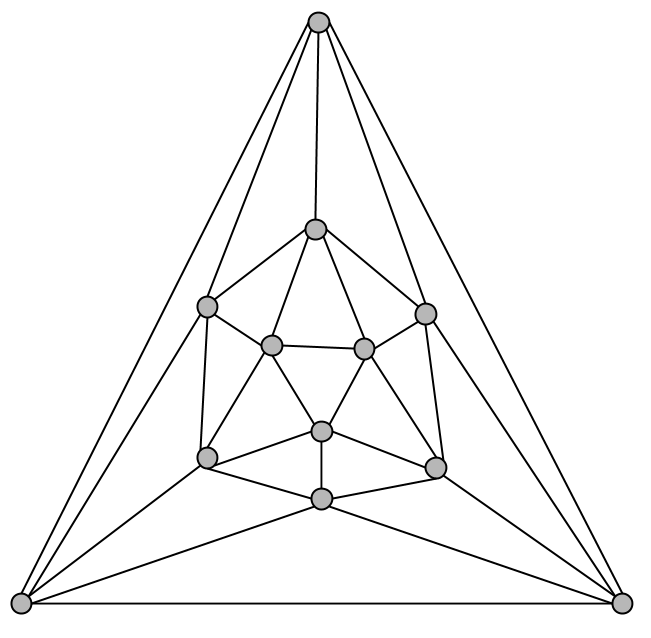
\includegraphics[width=7cm]{iko}
\end{center}
\caption{Der Ikosaeder hat 20 Facetten (gleichseitige Dreiecken), 30 Kanten und 12 Ecken.}
\end{figure}

\begin{figure}[htpb]
\begin{center}
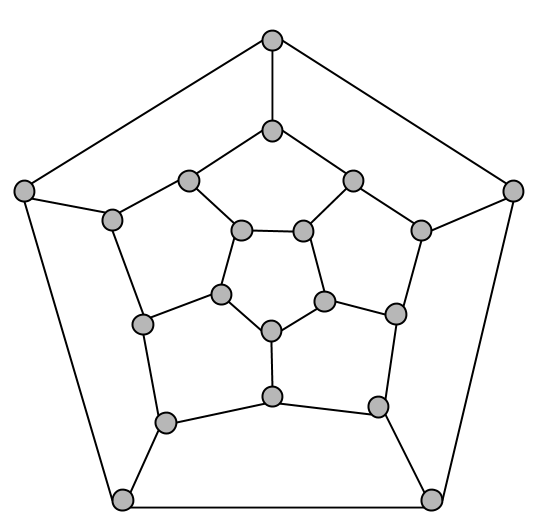
\includegraphics[width=7cm]{dode}
\end{center}
\caption{Der Dodekaeder hat 12 Facetten (regelmäßiges Fünfeck), 30 Kanten und 20 Ecken.}
\end{figure}




\end{task}


\begin{task}{d-dimensionale Polytope}
\item[]

$d$-dimensionaler Einheitswürfel $W_d$\\
\subtask{a}
Geben Sie die Ecken und die $d - 1$-dimensionalen Facetten von $W_d$ an.
Wieviele gibt es davon?
\subtask{b}
Zeichnen Sie den $W_4$ dh. seine Ecken und Kanten möglichst anschaulich.

$d$-dimensionaler Einheitssimplex $S_d$\\
\subtask{a}
Geben Sie die Ecken und die $d - 1$-dimensionalen Facetten von $S_d$ an
Wieviele gibt es davon?
\subtask{b}
Zeichnen Sie den $S_4$ dh. seine Ecken und Kanten möglichst anschaulich.


\end{task}

\begin{task}{Konvexe Hülle}
\item[]
Punkte einen nach dem anderen hinzuzufügen und konvexe Hülle aktualisieren klingt gut: Wenn der hinzukommende Punkt innerhalb bzw. auf dem Rand der kovexen Hülle liegt, dann muss man nichts tun, nur wenn er außerhalb liegt wird es interessant.

Von dem Punkt aus gesehen, würde ich das Ding in die Ebene projizieren. Flächen einfügen zwischen allen Kanten die auf dem entstanden Rand liegen und dem Punkt. Kanten zwischen allen Knoten auf Rand und Punkt hinzufügen

Der ganze Rest der nun verdeckt wird wegschmeißen.
\end{task}
\end{document}